\chapter{Implementación de Model2Blockly}
\label{chap:implementacion}

Este capítulo explica la implementación de Model2Blockly siguiendo el recorrido
de una ejecución completa. A diferencia del capítulo anterior, centrado en el
diseño y la arquitectura, aquí se identifican las tecnologías, clases y
operaciones que materializan cada etapa de la cadena generativa.

La exposición comienza mostrando cómo ejecutar la herramienta sobre el ejemplo
AppMaker y cómo localizar el editor obtenido. Después se presentan el flujo
interno, la organización del código y la carga y validación de las dos entradas.
Sobre esa base se detallan la ruta textual \texttt{.m2b}, el contrato y la
serialización del modelo intermedio \texttt{EditorSpec}, los adaptadores Java, el
generador HTML/JavaScript y el comportamiento en el navegador. El capítulo
termina con la integración y distribución en Eclipse, las entradas independientes y
las pruebas de implementación.

\section{Ejecución de Model2Blockly}
\label{sec:ejecucion-model2blockly}

Antes de detallar las clases internas, esta sección presenta el procedimiento
observable desde el punto de vista del usuario. La forma principal de ejecutar
Model2Blockly es mediante su plugin de Eclipse. El entorno debe iniciarse con
Java 21 y el plugin puede instalarse desde el repositorio p2 publicado por el
proyecto o ejecutarse desde el código fuente mediante una instancia runtime de
Eclipse. En ambos casos, la acción de generación se aplica a un fichero de
entrada situado en el workspace.

El ejemplo AppMaker incluido en el repositorio permite reproducir la ruta Ecore
mediante los siguientes pasos:

\begin{enumerate}
  \item abrir o importar el proyecto principal en Eclipse;
  \item seleccionar el fichero \path{model/app_maker.ecore};
  \item ejecutar \texttt{Model2Blockly -> Generate Blockly Editor} desde el menú
  contextual;
  \item revisar el informe \path{app_maker_generated/generation_report.html}
  que Eclipse abre al finalizar la generación;
  \item abrir
  \path{app_maker_generated/html/Appmaker_standalone.html} en un navegador para
  utilizar el editor generado.
\end{enumerate}

La ruta textual se ejecuta de la misma forma seleccionando
\path{examples/app_maker.m2b}. En los dos casos, si no se detectan errores, la
herramienta crea junto a la entrada un directorio con el sufijo
\texttt{\_generated}. El directorio contiene el informe de generación, una
serialización XMI de \texttt{EditorSpec}, las definiciones de bloques, la paleta,
los scripts de generación y validación, un modelo de ejemplo y las páginas HTML
del editor.

La Figura \ref{fig:appmaker-ecore-generation-report} muestra el informe que se
abre después de ejecutar la acción sobre \texttt{app\_maker.ecore}. En su parte
superior se identifican la entrada, el paquete Ecore, el número de bloques y
categorías, y las validaciones generadas. La tabla central permite comprobar que
la ejecución ha recorrido el modelo fuente, \texttt{EditorSpec}, su
serialización XMI y la generación del editor Blockly.

\begin{figure}[htbp]
  \centering
  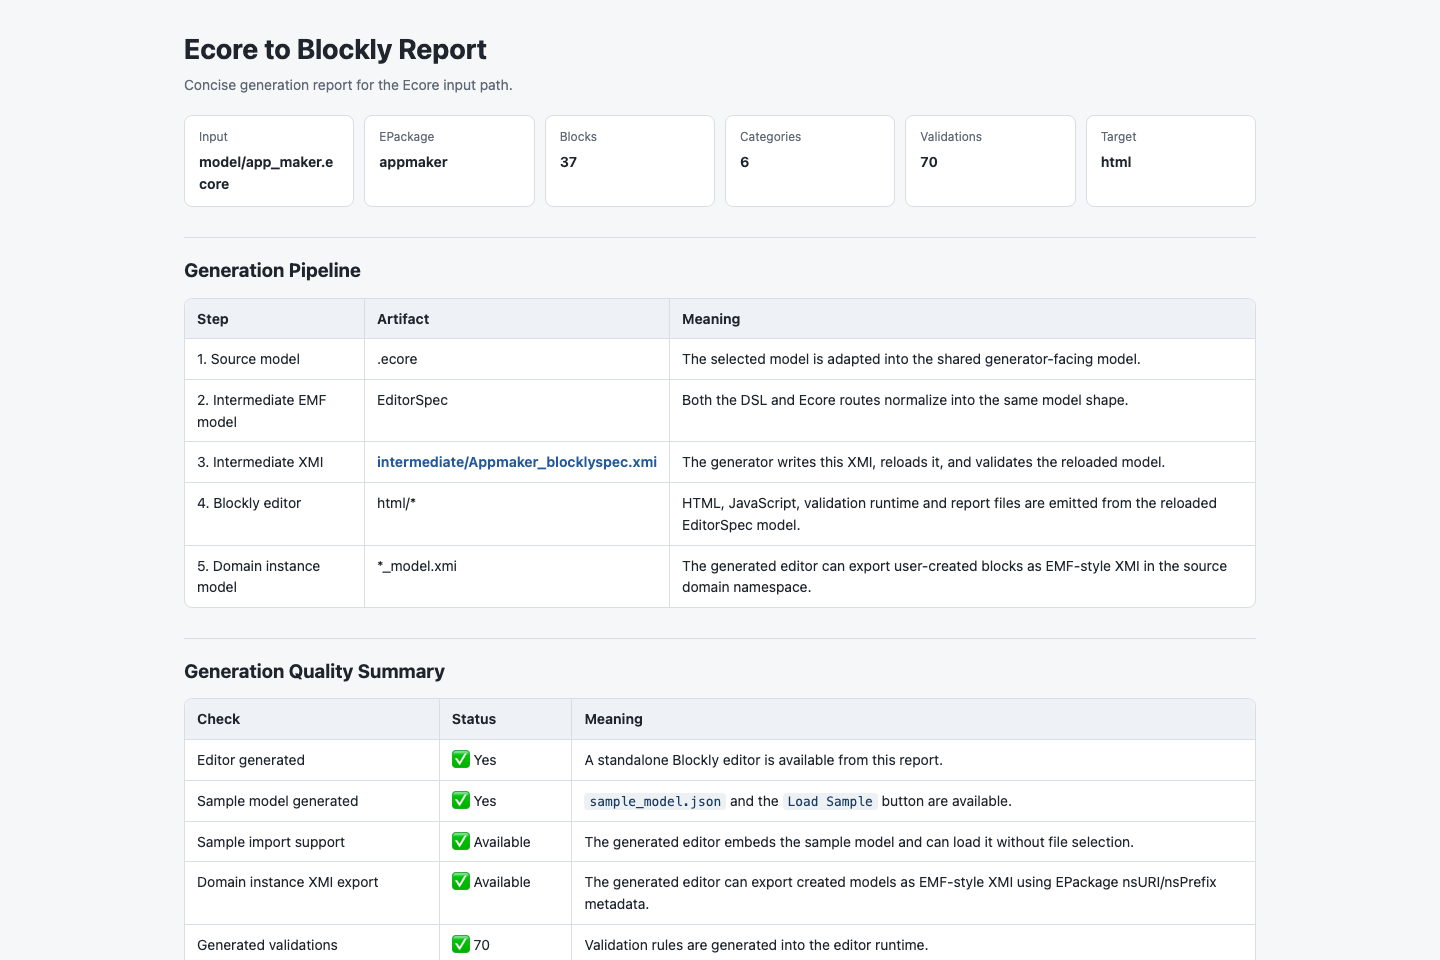
\includegraphics[width=0.90\textwidth,trim=150 300 150 30,clip]{assets/appmaker/appmaker-ecore-generation-report.png}
  \caption{Informe abierto después de generar el editor desde
  \texttt{app\_maker.ecore}}
  \label{fig:appmaker-ecore-generation-report}
\end{figure}

Conviene distinguir las dos ejecuciones implicadas. La primera se realiza en
Eclipse y transforma la descripción del dominio en artefactos web. La segunda se
realiza en el navegador al abrir la página autónoma
\texttt{*\_standalone.html}; en ella,
el usuario construye modelos del dominio mediante bloques, ejecuta las
validaciones generadas y exporta el resultado como JSON, XMI o código textual.
La Figura \ref{fig:appmaker-ecore-editor} muestra esta segunda ejecución con el
modelo de ejemplo cargado en el workspace.

\begin{figure}[htbp]
  \centering
  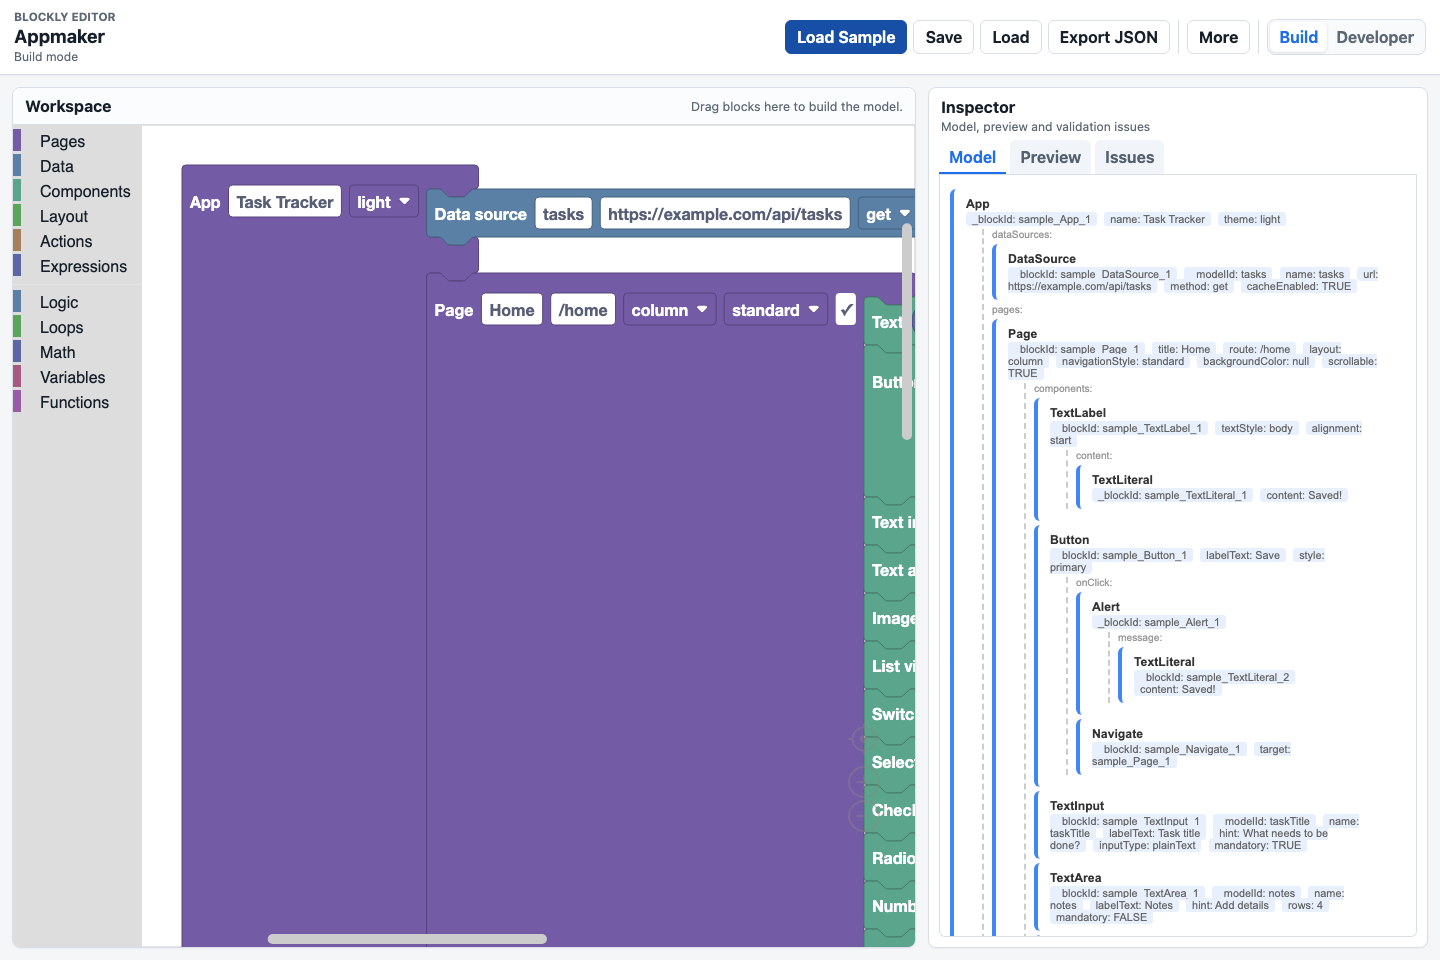
\includegraphics[width=\textwidth]{assets/appmaker/appmaker-ecore-editor.png}
  \caption{Editor Blockly ejecutado en el navegador después de la generación
  desde \texttt{app\_maker.ecore}}
  \label{fig:appmaker-ecore-editor}
\end{figure}

Las secciones siguientes abren esta cadena paso a paso y relacionan cada
operación visible con su implementación.

\section{Flujo interno de una ejecución}
\label{sec:flujo-interno-ejecucion}

En la ejecución integrada, la acción seleccionada por el usuario se atiende en
\texttt{GenerateBlocklyEditorHandler}. Esta clase determina la extensión del
fichero y elige una de las dos ramas de carga. La Figura
\ref{fig:flujo-interno-ejecucion} representa esta secuencia con los nombres de
los componentes implementados. No es una segunda arquitectura del sistema, sino
la traza concreta que sigue una petición de generación dentro del plugin.

\begin{figure}[htbp]
  \centering
  \resizebox{0.93\textwidth}{!}{%
  \begin{tikzpicture}[
      node distance=0.62cm and 1.15cm,
      box/.style={draw=black!55, rounded corners=2pt, minimum height=0.72cm,
        align=center, font=\small, inner sep=5pt},
      entrybox/.style={box, fill=black!5, text width=6.8cm},
      sourcebox/.style={box, fill=green!8, text width=4.1cm},
      routebox/.style={box, fill=blue!7, text width=4.1cm},
      commonbox/.style={box, fill=orange!10, text width=8.6cm},
      arrow/.style={-{Latex[length=2.4mm]}, thick, draw=black!70}
    ]
    \node[entrybox] (handler)
      {\texttt{GenerateBlocklyEditorHandler}\\selección de la ruta de entrada};

    \node[sourcebox, below left=of handler] (ecore)
      {Fichero \texttt{.ecore}};
    \node[sourcebox, below right=of handler] (dsl)
      {Fichero \texttt{.m2b}};

    \node[routebox, below=of ecore] (ecoreload)
      {\texttt{ResourceSet}\\+ \texttt{EPackage}};
    \node[routebox, below=of dsl] (dslload)
      {\texttt{XtextResource}\\+ \texttt{DomainModel}\\+ validación Xtext};

    \node[routebox, below=of ecoreload] (ecoreadapter)
      {\texttt{EcoreAdapter}\\implementado en Java};
    \node[routebox, below=of dslload] (dsladapter)
      {\texttt{DomainModelAdapter}\\implementado en Java};

    \path let \p1=(ecoreadapter), \p2=(dsladapter) in
      node[commonbox] (spec) at ($ (\p1)!0.5!(\p2) +(0,-1.35cm) $)
      {Modelo EMF común \texttt{EditorSpec}};
    \node[commonbox, below=of spec] (diagnostics)
      {\texttt{BlocklySpecDiagnostics}\\validación de la especificación común};
    \node[commonbox, below=of diagnostics] (xmi)
      {\texttt{BlocklySpecXmiSerializer}\\serialización, recarga y nueva validación};
    \node[commonbox, below=of xmi] (generator)
      {\texttt{BlocklyCodeGenerator} en Xtend\\generación modelo a texto};
    \node[commonbox, below=of generator] (output)
      {Directorio \texttt{\_generated}: informe, XMI intermedio,\\
       bloques, paleta, validaciones y páginas HTML};

    \draw[arrow] (handler) -- (ecore);
    \draw[arrow] (handler) -- (dsl);
    \draw[arrow] (ecore) -- (ecoreload);
    \draw[arrow] (dsl) -- (dslload);
    \draw[arrow] (ecoreload) -- (ecoreadapter);
    \draw[arrow] (dslload) -- (dsladapter);
    \draw[arrow] (ecoreadapter) -- (spec);
    \draw[arrow] (dsladapter) -- (spec);
    \draw[arrow] (spec) -- (diagnostics);
    \draw[arrow] (diagnostics) -- (xmi);
    \draw[arrow] (xmi) -- (generator);
    \draw[arrow] (generator) -- (output);
  \end{tikzpicture}%
  }
  \caption{Flujo interno implementado para una petición de generación}
  \label{fig:flujo-interno-ejecucion}
\end{figure}

En la rama Ecore, EMF carga el recurso y obtiene un \texttt{EPackage}; en la
rama textual, Xtext analiza, enlaza y valida el fichero antes de obtener un
\texttt{DomainModel}. Los adaptadores Java convierten ambos objetos en una
instancia de \texttt{EditorSpec}. A partir de ese punto, la ejecución es común:
se comprueba el modelo, se serializa como XMI, se vuelve a cargar y se valida de
nuevo antes de entregarlo al generador Xtend.

El generador devuelve un mapa de rutas y contenidos textuales. El manejador crea
el directorio de salida, escribe cada entrada del mapa y actualiza el workspace
de Eclipse. Esta última escritura explica por qué una única acción produce varios
ficheros relacionados y no solo la página autónoma mostrada en la sección
anterior. Las secciones posteriores detallan las operaciones resumidas en cada
caja de la figura.

\section{Organización del proyecto}
\label{sec:organizacion-proyecto}

La implementación se distribuye en tres bundles OSGi ejecutables creados según la
estructura habitual de Xtext \cite{xtextProject}. El proyecto
\path{io.github.plortinus.model2blockly} contiene la gramática, el modelo EMF
común, los adaptadores, la validación, los generadores y las entradas de línea de
comandos. El proyecto terminado en \path{.ide} aporta la configuración de los
servicios de lenguaje independientes de la interfaz. Finalmente, el proyecto
terminado en \path{.ui} registra el editor, los menús y los handlers que conectan
la generación con el workspace de Eclipse.

Otros dos proyectos no añaden lógica a la transformación. El proyecto
\path{.feature} agrupa los bundles instalables y \path{.updatesite} construye el
repositorio p2 utilizado para distribuir el plugin. Dentro de los tres bundles
ejecutables, la Tabla \ref{tab:paquetes-implementacion} relaciona cada componente
con los ficheros que materializan su implementación y con la tecnología empleada.

\begin{table}[H]
  \centering
  \small
  \setlength{\tabcolsep}{4pt}
  \begin{tabular}{@{}
      >{\raggedright\arraybackslash}p{0.17\textwidth}
      >{\raggedright\arraybackslash}p{0.40\textwidth}
      >{\raggedright\arraybackslash}p{0.32\textwidth}@{}}
    \toprule
    Componente & Implementación concreta & Función en la ejecución \\
    \midrule
    DSL textual & \texttt{Model2Blockly.xtext} (Xtext) y
    \texttt{Model2BlocklyValidator.java} (Java) & Analizar y validar una entrada
    \texttt{.m2b}. \\

    Modelo EMF común & \texttt{blockly\_editor\_spec.ecore} y código Java generado
    en \texttt{emf-gen} & Representar la especificación normalizada
    \texttt{EditorSpec}. \\

    Adaptadores & \texttt{EcoreAdapter.}\allowbreak\texttt{toEditorSpec}
    \allowbreak\texttt{(EPackage)} y
    \texttt{DomainModelAdapter.}\allowbreak\texttt{toEditorSpec}
    \allowbreak\texttt{(DomainModel)} (Java) & Recorrer cada
    modelo de entrada y construir el mismo \texttt{EditorSpec}. \\

    Diagnóstico y XMI & \texttt{BlocklySpecDiagnostics.java} y
    \texttt{BlocklySpecXmiSerializer.java} (Java) & Validar, serializar y volver a
    cargar el modelo común. \\

    Generación & \texttt{BlocklyCodeGenerator.xtend} (Xtend) y clases auxiliares
    del paquete \texttt{generator} (Java) & Producir HTML, JavaScript, JSON,
    informes y modelos de ejemplo. \\

    Integración Eclipse & \texttt{GenerateBlocklyEditor}\allowbreak
    \texttt{Handler.java} (Java) y \texttt{plugin.xml} & Registrar el comando,
    ejecutar la cadena y escribir sus resultados en el workspace. \\

    Ejecución standalone & Clases \texttt{*Main.java} del paquete
    \texttt{standalone} (Java) & Exponer la generación y el parcheado mediante
    línea de comandos. \\

    Pruebas & Clases \texttt{*Test.java} del directorio \texttt{test}
    (JUnit/Java) & Comprobar adaptadores, modelo común, validación y generación. \\
    \bottomrule
  \end{tabular}
  \caption{Organización de los componentes implementados}
  \label{tab:paquetes-implementacion}
\end{table}

En particular, la fila \emph{Adaptadores} corresponde a dos clases escritas
manualmente en Java, no a código de transformación generado por Xtext. Sus
métodos públicos reciben objetos EMF que ya han sido cargados: un
\texttt{EPackage} en la primera ruta y un \texttt{DomainModel} en la segunda.
Ambas clases recorren esos objetos mediante sus API tipadas y delegan la creación
final de la instancia EMF de \texttt{EditorSpec} en
\texttt{BlocklySpecModelMapper}. Las secciones
\ref{sec:implementacion-ecore-adapter} y
\ref{sec:implementacion-domainmodel-adapter} detallan las reglas aplicadas por
cada clase.

Esta organización materializa la arquitectura del capítulo anterior sin
repetirla: allí se justificaron los componentes y sus dependencias; aquí se
identifican las clases, los lenguajes y los artefactos que ejecutan esas
responsabilidades.

\section{Carga y validación de las entradas}
\label{sec:carga-validacion-entradas}

La carga se implementa antes de los adaptadores. \texttt{EcoreAdapter} recibe un
objeto EMF ya construido y \texttt{DomainModelAdapter} recibe el modelo tipado
producido por Xtext; ninguna de las dos clases abre ficheros. En la ejecución
desde Eclipse, esta responsabilidad reside en
\texttt{GenerateBlocklyEditorHandler}; las clases de entrada independiente reproducen el mismo
patrón para ficheros situados fuera del workspace. El resultado de esta etapa es
un \texttt{EPackage} o un \texttt{DomainModel} válido para iniciar la
transformación.

\subsection{Carga de un metamodelo \texttt{.ecore}}

El método \texttt{generateFromEcore} registra
\texttt{EcoreResourceFactoryImpl} para la extensión \texttt{ecore}, crea un
\texttt{ResourceSetImpl} y construye una URI de fichero a partir de la ubicación
del recurso seleccionado. La llamada \texttt{getResource(uri, true)} solicita la
carga inmediata del documento XMI y EMF resuelve sus elementos y referencias. El
primer objeto raíz se obtiene como \texttt{EPackage} y se entrega a
\texttt{EcoreAdapter}. La clase \texttt{EcoreToBlocklyMain} utiliza la misma
secuencia en su método \texttt{loadEPackage}.

Esta rama no utiliza el parser ni el validador de Xtext. Los problemas que
impiden leer el recurso se propagan como excepciones de carga; las restricciones
específicas que necesita el generador se comprueban después de la adaptación
mediante \texttt{BlocklySpecDiagnostics}. Esta separación evita interpretar
como sintaxis textual un metamodelo que ya dispone del formato estándar de EMF.

\subsection{Carga y validación de una entrada \texttt{.m2b}}

La ruta textual comienza registrando el lenguaje con
\texttt{Model2BlocklyStandalone}\allowbreak\texttt{Setup}. La configuración generada por Xtext
asocia el mismo lenguaje con las extensiones \texttt{.m2b} y
\texttt{.model2blockly}; la segunda se conserva por compatibilidad. El inyector
de Guice proporciona el \texttt{ResourceSet}, que carga el fichero como un
\texttt{XtextResource}. El parser crea el árbol EMF y el enlazador resuelve los
nombres usados para categorías, superclases y tipos. Si la carga termina
correctamente, el primer elemento del recurso debe ser una instancia de
\texttt{DomainModel}.

El Listado \ref{lst:carga-modelo-m2b} resume las llamadas Java que implementan
esta etapa en el manejador. La clase de entrada independiente
\texttt{Model2BlocklyToBlocklyMain} contiene la misma secuencia, cambiando
únicamente el origen de la ruta del fichero.

\begin{lstlisting}[language=Java, caption={Secuencia esencial de carga y validación de una entrada \texttt{.m2b}}, label={lst:carga-modelo-m2b}]
Injector injector = new Model2BlocklyStandaloneSetup()
    .createInjectorAndDoEMFRegistration();
ResourceSet resourceSet = injector.getInstance(ResourceSet.class);
Resource resource = resourceSet.getResource(fileUri, true);
XtextResource xtext = (XtextResource) resource;

xtext.validateConcreteSyntax();
Model2BlocklyValidationDiagnostics.throwIfSyntaxErrors(
    sourceLabel, resource.getErrors());
Model2BlocklyValidationDiagnostics.throwIfErrors(
    sourceLabel,
    xtext.getResourceServiceProvider().getResourceValidator()
        .validate(resource, CheckMode.ALL,
            CancelIndicator.NullImpl));

DomainModel domain =
    (DomainModel) resource.getAllContents().next();
\end{lstlisting}

La primera comprobación recoge los errores producidos durante el análisis y el
enlazado. A continuación, el \texttt{IResourceValidator} ejecuta en modo
\texttt{ALL} las reglas \texttt{@Check} de
\texttt{Model2BlocklyValidator}. Estas reglas detectan, entre otros casos,
nombres de clase duplicados, cardinalidades incoherentes, entradas de valor con
un tipo no válido, widgets incompatibles, referencias a campos inexistentes y
expresiones de validación no soportadas. El método \texttt{throwIfErrors} detiene
la generación únicamente ante diagnósticos de severidad \emph{error}; las
advertencias permanecen visibles en el editor, pero permiten continuar.

\subsection{Niveles de validación y comunicación de errores}

La implementación aplica tres niveles consecutivos. Primero se comprueba que el
recurso pueda cargarse y, en la ruta textual, que su sintaxis y sus referencias
sean correctas. Después se ejecutan las reglas semánticas específicas del DSL.
Finalmente, tras llamar al adaptador correspondiente,
\texttt{BlocklySpecDiagnostics.assertValid} comprueba las invariantes del
\texttt{EditorSpec} común. Esta última validación se repite después de serializar
y recargar el XMI, por lo que el generador solo recibe un modelo que ha superado
el contrato intermedio completo.

Cuando la ejecución se realiza en Eclipse, los errores semánticos y los
diagnósticos del modelo común se convierten en marcadores
\texttt{IMarker.PROBLEM} asociados al fichero y, cuando existe información de
origen, a su línea. El manejador vuelve a abrir la entrada y muestra un diálogo con
el resumen. En las entradas independientes, el mismo diagnóstico se escribe en la
salida de error y el proceso termina con un código distinto de cero. De este
modo, las dos formas de ejecución comparten las comprobaciones, aunque presentan
el resultado mediante interfaces diferentes.

\section{Ruta textual \texttt{.m2b} con Xtext}
\label{sec:implementacion-xtext}

La gramática Xtext define el lenguaje textual de entrada \texttt{.m2b} y
vincula sus reglas con los conceptos del metamodelo EMF asociado. A partir de
esta gramática, Xtext genera el parser y el soporte de edición
\cite{xtextProject,bettini2013xtext,bettini2015xsemantics}. Así, cada fichero
DSL puede tratarse como un modelo EMF. La raíz de ese modelo agrupa el nombre
del dominio, las opciones de generación, la configuración del workspace, las
categorías, las clases y las restricciones.

Las clases del dominio se declaran con una construcción específica del DSL. Cada
clase puede ser abstracta, generar un bloque de salida, heredar de otra clase,
pertenecer a una categoría, definir color, etiqueta, tooltip, disposición en
línea y plantilla de código. Dentro de una clase se declaran cuatro tipos de
elementos: atributos, contenciones, referencias y entradas de valor. Esta
distinción en la gramática se corresponde con las formas principales en las que
Blockly representa información: campos, entradas de sentencias, desplegables de
referencia y conectores de valor.

El DSL también incluye opciones de interfaz. Con estas opciones se pueden indicar
widgets, etiquetas, textos de ayuda, grupos,
orden de presentación, campos de solo lectura, campos ocultos y campos usados
para mostrar referencias. Esta información no es necesaria para un editor
Blockly básico, pero permite enriquecer la salida generada sin escribir
JavaScript a mano. En la memoria se usa para explicar la correspondencia con
Ecore y para mostrar una forma más compacta de definir el mismo lenguaje
AppMaker.

El Listado \ref{lst:appmaker-dsl} muestra un fragmento representativo de la
ruta textual \texttt{.m2b} aplicado al dominio AppMaker. En pocas líneas se
declaran una categoría, un bloque raíz, una contención con cardinalidad y un
bloque que referencia dinámicamente una fuente de datos. La misma información
acabaría convertida en campos, entradas y validaciones dentro del modelo
intermedio.

\begin{lstlisting}[caption={Fragmento representativo del DSL textual \texttt{.m2b} para AppMaker}, label={lst:appmaker-dsl}]
domain Appmaker codeLanguage "javascript" codeFileExtension "js"

category Pages label "Pages" colour 260
category Components label "Components" colour 160
category Data label "Data" colour 210

class App category Pages colour 260 label "App" {
  attribute name : string default "Task Tracker" required
    widget text uiLabel "App name" group "App" order 1
  contains DataSource dataSources [1..20]
    uiLabel "Data sources" group "Data" order 3
  contains Page pages [1..20]
    uiLabel "Pages" group "Pages" order 4
}

class ListView extends Component category Components colour 160 label "List view" {
  reference DataSource source required
    widget reference-select uiLabel "Source" referenceLabelField name
  value TextExpression itemTitle shadow TextLiteral
}
\end{lstlisting}

Una vez analizado el fichero como se explicó en la Sección
\ref{sec:carga-validacion-entradas}, el resultado de esta gramática es un
\texttt{DomainModel} enlazado y validado. Ese objeto constituye la entrada del
adaptador Java descrito posteriormente en la Sección
\ref{sec:implementacion-domainmodel-adapter}.

\section{Modelo intermedio EMF y vista Java}
\label{sec:implementacion-modelo-intermedio}

El contrato del modelo intermedio está definido como metamodelo EMF en el
fichero \texttt{blockly\_editor\_spec.ecore}, dentro del directorio
\texttt{model}. EMF genera a partir de él las interfaces Java
\texttt{EditorSpec}, \texttt{BlockTypeSpec}, \texttt{FieldSpec} y los demás
tipos del paquete \texttt{intermediate.blocklyspec}, junto con
\texttt{BlocklySpecFactory}. Para facilitar la construcción de esas instancias,
el proyecto conserva además \texttt{BlocklyEditorSpec}, una vista Java auxiliar del
mismo contenido. \texttt{BlocklySpecModelMapper} implementa la copia en ambos
sentidos entre esa vista y las instancias creadas por la factoría EMF.

El objeto EMF no se entrega directamente al generador después de la adaptación.
La serialización se encapsula en
\texttt{BlocklySpecXmi}\allowbreak\texttt{Serializer}. Esta clase crea un
\texttt{ResourceSet}\allowbreak\texttt{Impl} y registra
\texttt{BlocklySpecPackage.}\allowbreak\texttt{eNS\_URI} y añade el
\texttt{EditorSpec} a un \texttt{XMIResource}\allowbreak\texttt{Impl} con la
URI en memoria \texttt{memory:/}\allowbreak\texttt{blocklyspec.xmi}. El recurso se guarda en UTF-8, se vuelve a
cargar desde esa cadena y se comprueba que su raíz siga siendo un
\texttt{EditorSpec}. El Listado \ref{lst:ciclo-editor-spec-xmi} muestra cómo el
manejador aplica este ciclo en las dos rutas de entrada.

\begin{lstlisting}[language=Java, caption={Validación, serialización y recarga del modelo intermedio}, label={lst:ciclo-editor-spec-xmi}]
BlocklySpecDiagnostics.assertValid(intermediateModel, sourceLabel,
    sourceMapper);

String intermediateXmi =
    BlocklySpecXmiSerializer.toXmi(intermediateModel);
EditorSpec spec =
    BlocklySpecXmiSerializer.fromXmiToEditorSpec(intermediateXmi);

BlocklySpecDiagnostics.assertValid(
    spec, sourceLabel + " intermediate XMI");
Map<String, String> generated =
    new BlocklyCodeGenerator().generate(spec);
\end{lstlisting}

En el extracto, \texttt{sourceMapper} representa el mapeador creado por
\texttt{forEPackage} o \texttt{forDomainModel}, según la ruta. El primer
diagnóstico puede asociarse con elementos del modelo fuente mediante
\texttt{sourceMapper}; el segundo valida el objeto recargado. De este modo, un
error de serialización, una raíz incorrecta o la pérdida de un dato obligatorio
se detectan antes de generar texto. La misma cadena XMI se conserva después como
\path{intermediate/*_blocklyspec.xmi}, por lo que el artefacto inspeccionable es
exactamente el contenido usado para generar el editor.

Cada tipo de bloque guarda su forma de conexión: bloque raíz, bloque apilable,
bloque apilable tipado, bloque de valor o bloque de valor tipado. Esta
clasificación permite generar las conexiones visuales adecuadas sin mezclar
reglas específicas de Blockly con la lectura del dominio. La implementación
mantiene además listas separadas para campos, entradas de sentencias,
referencias y entradas de valor, lo que facilita generar cada tipo de elemento
con la construcción Blockly adecuada.

El modelo intermedio también conserva información de orden para las entradas de
un bloque. Esta decisión es relevante para la ruta Ecore: cuando las
características de una clase se leen desde el metamodelo, el orden
original de atributos y referencias puede influir en la legibilidad del bloque
generado. El generador usa esta lista cuando está disponible y, si no existe,
aplica un orden por defecto.

La ventaja de esta implementación es el desacoplamiento. Los adaptadores de
entrada producen una instancia conforme al mismo metamodelo intermedio, y los
generadores consumen su vista Java sin depender de cómo fue creada. Así, las
entradas y las salidas quedan separadas en el código, pero el contrato MDE sigue
siendo el metamodelo EMF y su serialización XMI.

\section{Adaptador desde Ecore}
\label{sec:implementacion-ecore-adapter}

Los dos adaptadores se implementan como clases Java ordinarias con métodos
estáticos; no se instancian ni contienen plantillas de generación. El Listado
\ref{lst:entrada-adaptadores-java} muestra sus puntos de entrada reales. Cada
método realiza primero una normalización hacia \texttt{BlocklyEditorSpec}, una
vista Java interna formada por listas y objetos tipados, y después invoca
\texttt{BlocklySpecModelMapper.toEmfSpec}. Este segundo paso usa
\texttt{BlocklySpecFactory.eINSTANCE} para crear el \texttt{EditorSpec} definido
por el metamodelo común y copiar recursivamente categorías, bloques, campos,
entradas, validaciones y opciones de workspace. Por tanto, la vista Java es un
objeto auxiliar de construcción; el resultado contractual del adaptador es la
instancia EMF \texttt{EditorSpec}.

\begin{lstlisting}[float=htbp, language=Java, caption={Puntos de entrada Java de los dos adaptadores}, label={lst:entrada-adaptadores-java}]
// EcoreAdapter.java
public static EditorSpec toEditorSpec(EPackage pkg) {
    return BlocklySpecModelMapper.toEmfSpec(fromEPackage(pkg));
}

// DomainModelAdapter.java
public static EditorSpec toEditorSpec(DomainModel domain) {
    return BlocklySpecModelMapper.toEmfSpec(fromDomainModel(domain));
}
\end{lstlisting}

En la ruta Ecore, \texttt{fromEPackage} recibe el objeto obtenido durante la
carga descrita en la Sección \ref{sec:carga-validacion-entradas}. El método copia
primero el nombre, \texttt{nsURI}, prefijo y opciones globales del paquete.
Después reúne los nombres de las clases que son destino de alguna referencia de
contención; este conjunto se usa más adelante para distinguir bloques raíz de
bloques que deben conectarse como hijos. A continuación recorre todos los
\texttt{EClassifier} del paquete y de sus subpaquetes, selecciona los
\texttt{EClass} y llama a \texttt{convertEClass}. Este proceso usa directamente
la API de EMF: clases, atributos, referencias, herencia y cardinalidades
\cite{emfOverview}.

Desde el punto de vista de MDE, este adaptador es una transformación de modelos
implementada en Java sobre la API de EMF. No se ha usado un lenguaje específico
de transformación como ATL o ETL. La razón es pragmática: el generador debe
integrarse dentro de un plugin Eclipse/Xtext, reutilizar utilidades Java del
proyecto, emitir diagnósticos concretos sobre el fichero de entrada y construir
la instancia EMF \texttt{EditorSpec} que después se serializa como XMI. La
implementación queda así dentro de la misma cadena Java que carga el recurso y
comunica los errores al entorno Eclipse. La Tabla
\ref{tab:transformacion-ecore-editor-spec} resume las reglas principales de la
transformación.

El mapeo estructural se implementa de forma automática. Un atributo Ecore se
transforma en un campo visual; su tipo determina si el campo Blockly será
textual, numérico, booleano, desplegable, color, ángulo o imagen. Una referencia
de contención se transforma en una entrada estructural, porque representa una
relación jerárquica entre elementos del modelo. Una referencia no contenida se
transforma en una referencia dinámica, porque apunta a otro elemento ya
existente. Las cardinalidades se convierten en reglas de validación para que el
editor generado pueda avisar al usuario si faltan elementos obligatorios, si se
supera un límite superior o si un campo requerido queda sin completar.

La inferencia de conexiones también se realiza en el adaptador. Las clases
contenedoras que no están contenidas por otras pueden convertirse en bloques
raíz sin conexión vertical. Las clases que heredan de una superclase pueden
generar conexiones tipadas. Las clases marcadas como bloques de salida generan
conectores de valor. Esta inferencia es importante porque evita que el usuario
tenga que escribir a mano reglas de conexión Blockly para cada clase.

\begin{table}[H]
  \centering
  \small
  \begin{tabular}{|L{0.30\textwidth}|L{0.30\textwidth}|L{0.26\textwidth}|}
    \hline
    Elemento Ecore de entrada & Elemento \texttt{EditorSpec} destino & Uso en Blockly \\
    \hline
    \texttt{EPackage} & \texttt{EditorSpec} con nombre, \texttt{nsURI} y opciones
    globales & Identidad del editor y exportación XMI. \\
    \texttt{EClass} concreta & \texttt{BlockTypeSpec} & Tipo de bloque disponible en
    la paleta. \\
    \texttt{EClass} abstracta & \texttt{BlockTypeSpec} abstracto & Tipo usado para
    conexiones, pero no instanciable. \\
    \texttt{EAttribute} & \texttt{FieldSpec} & Campo de texto, número, booleano,
    color, ángulo o desplegable. \\
    \texttt{EReference containment=true} & \texttt{StatementInputSpec} & Entrada
    vertical para bloques hijos. \\
    \texttt{EReference containment=false} & \texttt{ReferenceFieldSpec} & Desplegable
    dinámico hacia elementos existentes. \\
    \texttt{lowerBound}/\texttt{upperBound} & \texttt{ValidationSpec} y límites de
    entrada & Avisos de obligatoriedad y cardinalidad. \\
    \texttt{EAnnotation} & Metadatos de bloque, interfaz, validación o código &
    Color, categoría, etiqueta, tooltip, widget y plantilla. \\
    \hline
  \end{tabular}
  \caption{Transformación principal de Ecore a \texttt{EditorSpec}}
  \label{tab:transformacion-ecore-editor-spec}
\end{table}

El adaptador permite enriquecer la generación mediante anotaciones Ecore. Las
anotaciones con fuente \texttt{blockly} afectan a la sintaxis visual: etiqueta,
color, categoría, tooltip, disposición en línea, bloque de salida, rangos
numéricos, entradas de valor o shadow blocks. Las anotaciones con fuente
\texttt{ui} se incorporan al modelo intermedio para personalizar la salida HTML. Las
anotaciones con fuente \texttt{code} permiten definir lenguaje, extensión de
archivo y plantillas de generación. Así, un metamodelo sin anotaciones puede
generar un editor básico, mientras que un metamodelo anotado puede producir una
experiencia más adaptada al dominio.

El Listado \ref{lst:appmaker-ecore} muestra el mismo tipo de información en la
ruta Ecore. El metamodelo conserva las clases y referencias EMF, y las
anotaciones añaden la sintaxis visual, la regla de validación y la plantilla de
código usadas por el generador.

\begin{lstlisting}[caption={Fragmento de \texttt{model/app\_maker.ecore} con anotaciones}, label={lst:appmaker-ecore}]
<eClassifiers xsi:type="ecore:EClass" name="Navigate" eSuperTypes="#//Action">
  <eAnnotations source="blockly">
    <details key="colour" value="30"/>
    <details key="category" value="Actions"/>
    <details key="inputsInline" value="true"/>
  </eAnnotations>
  <eAnnotations source="validation">
    <details key="mustFollow" value="Alert"/>
  </eAnnotations>
  <eAnnotations source="code">
    <details key="template" value="navigate(&quot;{{target}}&quot;);"/>
  </eAnnotations>
  <eStructuralFeatures xsi:type="ecore:EReference" name="target"
      lowerBound="1" eType="#//Page">
    <eAnnotations source="ui">
      <details key="widget" value="reference-select"/>
      <details key="label" value="Target page"/>
      <details key="referenceLabelField" value="title"/>
    </eAnnotations>
  </eStructuralFeatures>
</eClassifiers>
\end{lstlisting}

\section{Adaptador desde la ruta textual \texttt{.m2b}}
\label{sec:implementacion-domainmodel-adapter}

El adaptador de la ruta textual también está implementado manualmente en Java.
\texttt{DomainModelAdapter.fromDomainModel} recibe la raíz EMF producida por
Xtext y ejecuta, en orden, los métodos \texttt{convertCategories},
\texttt{convertClasses}, \texttt{convertConstraints},
\texttt{convertValidations} y \texttt{convertWorkspaceOptions}. Después genera
las validaciones inferidas de cardinalidad, obligatoriedad y unicidad. El objeto
Java resultante vuelve al método \texttt{toEditorSpec} del Listado
\ref{lst:entrada-adaptadores-java}, donde se convierte al mismo modelo EMF común
que en la ruta Ecore.

El mapeo es más directo que en Ecore porque la gramática ya distingue los
conceptos específicos que necesita Model2Blockly. Los atributos se convierten en
campos, las contenciones en entradas estructurales, las referencias en
desplegables dinámicos y las entradas de valor en conexiones horizontales. Las
restricciones de orden se convierten en validaciones, y los campos marcados como
obligatorios generan comprobaciones de obligatoriedad.

La conversión de cada clase se implementa con un recorrido de la lista
\texttt{Feature} generada por Xtext. El Listado
\ref{lst:despacho-domainmodel-adapter} muestra el despacho esencial. Cada tipo
concreto se entrega a un método especializado y el nombre de la entrada se añade
a \texttt{orderedInputNames}; de este modo, el orden escrito en el fichero
\texttt{.m2b} se conserva al construir el bloque.

\begin{lstlisting}[language=Java, caption={Despacho de elementos del DSL en \texttt{DomainModelAdapter}}, label={lst:despacho-domainmodel-adapter}]
for (Feature feature : cls.getFeatures()) {
    if (feature instanceof Attribute) {
        FieldSpec field = convertAttribute((Attribute) feature);
        bt.getFields().add(field);
        bt.getOrderedInputNames().add(field.getName());
    } else if (feature instanceof Containment) {
        StatementInputSpec input =
            convertContainment((Containment) feature);
        bt.getStatementInputs().add(input);
        bt.getOrderedInputNames().add(input.getName());
    } else if (feature instanceof Reference) {
        ReferenceFieldSpec reference =
            convertReference((Reference) feature);
        bt.getReferenceFields().add(reference);
        bt.getOrderedInputNames().add(reference.getName());
    } else if (feature instanceof ValueInput) {
        ValueInputSpec input = convertValueInput((ValueInput) feature);
        bt.getValueInputs().add(input);
        bt.getOrderedInputNames().add(input.getName());
    }
}
\end{lstlisting}

\begin{table}[htbp]
  \centering
  \small
  \begin{tabular}{|L{0.30\textwidth}|L{0.30\textwidth}|L{0.26\textwidth}|}
    \hline
    Elemento del DSL & Elemento \texttt{EditorSpec} destino & Uso en Blockly \\
    \hline
    \texttt{domain} & \texttt{EditorSpec} & Nombre del editor y opciones de
    generación. \\
    \texttt{category} & \texttt{CategorySpec} & Categoría de la paleta y color por
    defecto. \\
    \texttt{class} & \texttt{BlockTypeSpec} & Tipo de bloque. \\
    \texttt{attribute} & \texttt{FieldSpec} & Campo visual del bloque. \\
    \texttt{contains [m..n]} & \texttt{StatementInputSpec} y
    \texttt{ValidationSpec} & Entrada de hijos y comprobación de cardinalidad. \\
    \texttt{reference} & \texttt{ReferenceFieldSpec} & Desplegable dinámico. \\
    \texttt{value} & \texttt{ValueInputSpec} & Entrada horizontal para bloques de
    valor. \\
    \texttt{must follow} & \texttt{ValidationSpec} & Regla local de orden. \\
    \hline
  \end{tabular}
  \caption{Normalización del DSL textual \texttt{.m2b} a \texttt{EditorSpec}}
  \label{tab:transformacion-dsl-editor-spec}
\end{table}

La implementación usa también información de herencia para determinar la forma
de conexión. Una clase marcada como bloque de salida se convierte en bloque de
valor; una clase con superclase genera conexiones tipadas; una clase con
contenciones y sin superclase puede funcionar como bloque raíz; y una clase
ordinaria se genera como bloque apilable. De este modo, la semántica declarada
en la sintaxis textual se transforma en reglas visuales de Blockly sin que el
autor del dominio tenga que conocer la API de bajo nivel de la biblioteca.

La estructura principal se lee con los tipos Java generados por Xtext
(\texttt{ClassDef}, \texttt{Attribute}, \texttt{Containment},
\texttt{Reference} y \texttt{ValueInput}). Solo algunas opciones de interfaz,
código y workspace se obtienen dinámicamente con
\texttt{eClass().getEStructuralFeature} y \texttt{eGet}. Esta decisión permite
que metadatos añadidos recientemente a la gramática puedan leerse antes de
regenerar todos los accesores, sin renunciar a la comprobación estática en el
recorrido estructural que determina los bloques.

\section{Generador HTML/JavaScript}
\label{sec:implementacion-generador-html}

El generador de la salida HTML/JavaScript transforma el modelo intermedio en los
artefactos necesarios para abrir el editor en un navegador: bloques, paleta,
exportación, validaciones, página de edición, página autónoma, workspace de
validaciones, modelo de ejemplo e informe de generación. Esta salida usa Blockly
para definir bloques, inyectar el workspace, gestionar la paleta, serializar y
generar código \cite{blocklyDocs}.

La generación de código se implementa principalmente en Xtend. La clase
principal, \texttt{Blockly\allowbreak{}Code\allowbreak{}Generator.xtend}, recibe
un \texttt{EditorSpec} y produce un mapa ordenado de nombres de fichero a
contenido textual. El Listado \ref{lst:entrada-generador-xtend} reproduce el
método de entrada: cada función \texttt{generate*} devuelve una cadena y el mapa
conserva la relación entre esa cadena y su fichero de destino.

\begin{lstlisting}[captionpos=t, caption={Método de entrada de \texttt{BlocklyCodeGenerator.xtend}}, label={lst:entrada-generador-xtend}]
def Map<String, String> generate(EditorSpec spec) {
    val files = new LinkedHashMap<String, String>()
    val base = spec.domainName ?: "domain"
    files.put(base + "_blocks.js", generateBlocksJs(spec))
    files.put(base + "_toolbox.js", generateToolboxJs(spec))
    files.put(base + "_generators.js", generateGeneratorsJs(spec))
    files.put(base + "_validations.js", generateValidationsJs(spec))
    files.put(base + "_editor.html", generateEditorHtml(spec))
    files.put(base + "_standalone.html", generateStandaloneHtml(spec))
    files.put("validation_workspace.html",
        ValidationWorkspaceHtmlGenerator.generate(spec))
    files.put("validation_blocks.json",
        ValidationBlockModelGenerator.generate(spec))
    files.put("validation_runtime.js",
        ValidationRuntimeGenerator.generateClassicJs(spec))
    files.put("sample_model.json", SampleModelGenerator.generate(spec))
    return files
}
\end{lstlisting}

Xtend se usa como mecanismo de generación porque se integra bien con Xtext y
permite escribir plantillas de
texto legibles dentro del proyecto Eclipse. No se ha usado Acceleo ni un motor
externo de plantillas. Algunas piezas auxiliares, como el modelo de ejemplo, el
runtime de validaciones y la vista visual de reglas, se implementan en clases
Java separadas para mantener responsabilidades acotadas.

El mapa no escribe directamente en disco. El
\texttt{GenerateBlocklyEditorHandler} antepone \texttt{html/} a sus rutas y
añade tres resultados producidos fuera de Xtend: el XMI intermedio, el
\texttt{README.md} y el informe de generación. Finalmente,
\texttt{writeFiles} crea los \texttt{IFile} del workspace y actualiza el proyecto.
Esta separación permite reutilizar el mismo generador desde las entradas
standalone sin depender de la API de Eclipse.

La generación de bloques comienza en \texttt{generateBlocksArray}, que filtra
los tipos concretos y llama a \texttt{blockTypeToBlockJson}. Este método crea
mapas de campos, referencias y entradas, y recorre
\texttt{orderedInputNames} para conservar el orden establecido por el
adaptador. Cada elemento se delega en \texttt{fieldToArg},
\texttt{referenceToArg}, \texttt{valueInputToArg} o
\texttt{statementInput}\allowbreak\texttt{ToArg}. Finalmente, un
\texttt{switch} sobre \texttt{Connection}\allowbreak\texttt{Type} emite
\texttt{previous}\allowbreak\texttt{Statement},
\texttt{nextStatement} u \texttt{output} con tipo libre o tipado. Las clases
abstractas quedan en el modelo para resolver herencia y conexiones, pero no se
incluyen como bloques instanciables.

La generación de la paleta produce el conjunto de bloques disponible para el
usuario. Si no hay categorías, el generador puede emitir una paleta simple. Si
existen categorías, genera una paleta categorizada, incluyendo subcategorías cuando se
han definido. También se incluyen categorías integradas de Blockly, como lógica,
bucles, matemáticas, variables y funciones, para que los dominios puedan
combinar bloques propios con construcciones generales cuando sea necesario.

Se generan dos envoltorios HTML sobre esos mismos contenidos. La página
\texttt{*\_editor.}\allowbreak\texttt{html} carga por separado los ficheros de bloques, paleta,
generadores y validaciones, lo que facilita incrustarla y depurar cada módulo.
La página \texttt{*\_standalone.html} incrusta el JavaScript específico del
dominio en un único documento para simplificar la demostración. En ambos casos,
la biblioteca Blockly y su generador JavaScript se cargan desde la CDN indicada
en las etiquetas \texttt{script}; por ello, la página autónoma no contiene una
copia local de Blockly y requiere acceso a esa dependencia al abrirse.

La Tabla \ref{tab:artefactos-generados} resume los ficheros principales que
emite la cadena generativa. Esta lista permite interpretar la salida como un
resultado reproducible y no como una única página HTML aislada.

\begin{table}[htbp]
  \centering
  \small
  \begin{tabular}{|L{0.32\textwidth}|L{0.54\textwidth}|}
    \hline
    Artefacto generado & Contenido \\
    \hline
    \texttt{html/*\_blocks.js} & Definiciones de bloques Blockly. \\
    \texttt{html/*\_toolbox.js} & Categorías y paleta del editor. \\
    \texttt{html/*\_generators.js} & Funciones de serialización y generación de
    código por bloque. \\
    \texttt{html/*\_validations.js} & Reglas de validación ejecutadas sobre el
    workspace. \\
    \texttt{html/*\_editor.html} & Página embebible del editor generado. \\
    \texttt{html/*\_standalone.html} & Página única que incrusta el código del
    dominio y carga Blockly desde CDN. \\
    \texttt{html/sample\_model.json} & Modelo de ejemplo usado por el botón
    \texttt{Load Sample}. \\
    \path{html/validation_workspace.html} & Editor visual de reglas de
    validación. \\
    \path{html/validation_blocks.json} & Árbol serializado de bloques de
    validación. \\
    \path{html/validation_runtime.js} & Compilación y evaluación de las reglas
    visuales en el navegador. \\
    \path{intermediate/*_blocklyspec.xmi} & Instancia XMI de
    \texttt{EditorSpec} recargada antes de generar HTML. \\
    \texttt{generation\_report.html} & Informe de trazabilidad de la generación. \\
    \texttt{README.md} & Instrucciones para abrir y revisar los resultados. \\
    \hline
  \end{tabular}
  \caption{Artefactos principales emitidos por la cadena generativa}
  \label{tab:artefactos-generados}
\end{table}

Entre esos artefactos, la exportación tiene dos objetivos. Por un lado,
serializa el workspace como una estructura JSON con el tipo de bloque,
identificador, campos, referencias, valores y sentencias. También puede exportar
ese contenido como XMI de instancia del dominio, usando el prefijo y el URI del
paquete de entrada y evitando mezclar ese XMI con el XMI intermedio
\texttt{EditorSpec}. Por otro lado, incorpora una ruta de generación de código
basada en plantillas. Si un bloque define una plantilla, el generador sustituye
marcadores por valores de campos, entradas de valor o secuencias de sentencias.
Si no existe plantilla, se usa una representación textual genérica. Esta
estrategia mantiene la exportación operativa incluso cuando el dominio todavía
no ha definido una semántica de código completa.

\section{Validaciones y referencias en tiempo de ejecución}
\label{sec:implementacion-validaciones-referencias}

La implementación distingue entre validación estática del DSL y validación en
tiempo de ejecución del editor generado. La primera se realiza en Eclipse/Xtext
antes de generar. La segunda se ejecuta en el navegador sobre el workspace
Blockly.

\texttt{generateValidationsJs} produce las funciones
\texttt{computeValidation}\allowbreak\texttt{Warnings},
\texttt{applyValidation}\allowbreak\texttt{Warnings} e
\texttt{init}\allowbreak\texttt{Validations}. La primera recorre
\texttt{workspace.}\allowbreak\texttt{getAllBlocks(false)} y evalúa las reglas aplicables a cada
tipo. Las reglas de orden consultan \texttt{getPreviousBlock}; las de
cardinalidad siguen la cadena iniciada en \texttt{getInputTargetBlock}; y las de
obligatoriedad y unicidad leen y comparan los valores de campo. La segunda
función agrupa los mensajes por bloque, llama a \texttt{setWarningText} y
actualiza el panel de problemas. \texttt{init}\allowbreak\texttt{Validations} registra finalmente un
listener para repetir el cálculo después de crear, borrar, mover o modificar un
bloque.

Las reglas se representan también como árboles en
\texttt{validation\_blocks.json}. La clase Java
\texttt{ValidationRuntimeGenerator} transforma cada árbol en una expresión de
runtime y genera \texttt{validation\_runtime.js}. En el navegador,
\texttt{createValidationAccessors} ofrece operaciones acotadas como
\texttt{value}, \texttt{has}, \texttt{inputCount}, \texttt{fieldUnique} y
\texttt{previousBlockIs}; \texttt{evaluateRuntimeExpression} ejecuta la
expresión con esos accesores. Esta representación permite que
\texttt{validation\_workspace.html} muestre las mismas reglas que utiliza el
editor, en lugar de mantener una segunda definición visual independiente.

Las referencias no contenidas se implementan como campos cuyos valores son
identificadores de bloques. La función generada
\texttt{updateReferenceDropdowns} agrupa las instancias existentes por tipo,
construye para cada destino una pareja etiqueta--identificador y sustituye las
opciones del desplegable. La etiqueta se toma del
\texttt{referenceLabelField}, del campo \texttt{name} o, como último recurso,
del tipo y una parte del identificador. Si se elimina el bloque referenciado, el
valor deja de estar entre las opciones válidas y se limpia.

Esta implementación mantiene la diferencia entre contención y referencia. Una
contención crea estructura jerárquica en el workspace, mientras que una
referencia selecciona un elemento que ya existe. La separación conserva la
información relacional del modelo de dominio.

Cuando existe una referencia opuesta, \texttt{synchronizeOppositeReferences}
calcula los valores inversos y actualiza el bloque destino. Una bandera
\texttt{\_\_syncingOpposite}\allowbreak\texttt{References} y la desactivación temporal de eventos
evitan que esa escritura genere un ciclo de notificaciones. El Listado
\ref{lst:listener-runtime-blockly} resume el listener compartido que mantiene
referencias, validaciones y vista de salida después de cada cambio estructural.

\begin{lstlisting}[caption={Actualización reactiva del editor generado}, label={lst:listener-runtime-blockly}]
workspace.addChangeListener(function(event) {
    if (event.type === Blockly.Events.BLOCK_MOVE ||
        event.type === Blockly.Events.BLOCK_CREATE ||
        event.type === Blockly.Events.BLOCK_DELETE ||
        event.type === Blockly.Events.BLOCK_CHANGE) {
        updateReferenceDropdowns(workspace);
        synchronizeOppositeReferences(workspace, event);
        if (typeof applyValidationWarnings === 'function')
            applyValidationWarnings(workspace);
        if (typeof updateOutput === 'function') updateOutput();
    }
});
\end{lstlisting}

Antes de exportar JSON, XMI o código, \texttt{confirmExportIfInvalid} vuelve a
ejecutar las validaciones y solicita confirmación si quedan advertencias. El
usuario puede por tanto inspeccionar un modelo incompleto sin bloquear la
edición, pero la exportación no oculta sus problemas. Los límites numéricos
\texttt{min} y \texttt{max} se incorporan directamente a los campos Blockly.

La página incluye además un ejecutor genérico de inspección.

El método \texttt{generateRuntimeScript} genera su código a partir del modelo.
Durante la ejecución, este código convierte el workspace a la
representación JSON del dominio, recorre recursivamente sus nodos y resalta el bloque visitado
con controles de ejecución, pausa y paso. No ejecuta la semántica particular de
cada dominio; sirve para observar la estructura construida y comprobar el orden
de recorrido del modelo.

El ciclo de validación se completa con una utilidad de parche. Desde línea de
comandos puede ejecutarse sobre un fichero
\texttt{validation\_blocks.edited.json} y desde Eclipse está expuesta como
\texttt{Apply Validation Blocks to Source}. El parche se aplica de forma
conservadora: solo actualiza reglas que se pueden mapear de manera inequívoca a
la sintaxis textual o a anotaciones Ecore, y deja fuera expresiones que no tengan
una traducción directa.

El comportamiento generado sigue siendo deliberadamente ligero. No constituye
un motor OCL completo ni un verificador semántico general. Cubre cardinalidad,
obligatoriedad, unicidad, referencias opuestas, expresiones declaradas y el
subconjunto de invariantes OCL que los adaptadores pueden traducir a los
accesores disponibles en JavaScript.

\section{Integración con Eclipse y distribución}
\label{sec:implementacion-eclipse-distribucion}

La integración con Eclipse se declara en el fichero \texttt{plugin.xml} del
bundle de interfaz. Este fichero registra los comandos
\texttt{generateBlocklyEditor} y \texttt{applyValidationPatch}, los asocia con
\texttt{GenerateBlocklyEditorHandler} y
\texttt{ApplyValidationPatchHandler}, y limita su visibilidad a selecciones de
un único fichero compatible. Las contribuciones al menú contextual incluyen
\texttt{.ecore} y \texttt{.m2b}; la extensión histórica
\texttt{.model2blockly} se conserva para poder abrir proyectos anteriores.

\texttt{GenerateBlocklyEditorHandler} extiende \texttt{AbstractHandler}. Su
método \texttt{execute} obtiene el \texttt{IFile} seleccionado y delega el
trabajo en un \texttt{IRunnableWithProgress} ejecutado por el servicio de
progreso de Eclipse. Dentro de ese runnable se selecciona la ruta Ecore o la
ruta textual. A continuación se reutilizan la carga de la Sección
\ref{sec:carga-validacion-entradas}, los adaptadores de las Secciones
\ref{sec:implementacion-ecore-adapter} y
\ref{sec:implementacion-domainmodel-adapter}, y el generador de la Sección
\ref{sec:implementacion-generador-html}. El resultado es el mapa de artefactos
que recibe \texttt{writeFiles}; este método crea de forma
recursiva el directorio \texttt{*\_generated}, convierte cada contenido a UTF-8
y usa \texttt{IFile.create} o \texttt{IFile.setContents} según exista o no el
recurso. Al terminar, el proyecto se refresca y se abre
\texttt{generation\_report.html} en el workbench.

La integración también traduce los fallos de la transformación al mecanismo de
diagnósticos del IDE. Si falla la validación de \texttt{EditorSpec}, el
\texttt{BlocklySpecSourceMapper} permite crear un \texttt{IMarker.PROBLEM} sobre
el elemento de origen, incluyendo línea, ubicación, mensaje y sugerencia cuando
están disponibles. Los errores producidos por Xtext se convierten del mismo modo
en marcadores asociados al fichero \texttt{.m2b}. Por tanto, el usuario no recibe
solamente una excepción Java: el editor de origen se abre y Eclipse muestra la
ubicación del problema.

\texttt{ApplyValidationPatchHandler} implementa el camino inverso para las
reglas editadas visualmente. El manejador propone los ficheros
\texttt{validation\_blocks.json} de la salida correspondiente, ejecuta primero
\texttt{ValidationPatchService.dryRun} y presenta los cambios antes de pedir
confirmación. Solo después ejecuta \texttt{apply}, refresca el recurso y vuelve
a abrir la fuente. Cuando la escritura se realiza sobre el mismo fichero, el
servicio conserva previamente una copia con extensión \texttt{.bak}.

La distribución instalable se materializa en dos niveles. El fichero
\texttt{feature.xml} agrupa los bundles principal, IDE y UI en la feature
\path{io.github.plortinus.model2blockly.feature}. Después,
\texttt{category.xml} publica esa feature en la categoría Model2Blockly del
repositorio p2. Este repositorio contiene los JAR de los tres bundles y los
metadatos \texttt{content.jar} y \texttt{artifacts.jar}; de esta forma, la misma
implementación descrita en este capítulo puede instalarse mediante
\texttt{Help -> Install New Software} sin importar los proyectos fuente.

El repositorio publica también el código fuente, el repositorio p2 y dos
demostraciones de AppMaker. Las fuentes son \path{model/app_maker.ecore} y
\path{examples/app_maker.m2b}; las salidas versionadas de
\path{examples/generated/} incluyen el informe, el XMI intermedio, el modelo de
ejemplo, las reglas de validación y el editor. Así pueden inspeccionarse sin
repetir la transformación. La Tabla \ref{tab:artefactos-entrega} reúne los
puntos de acceso utilizados para la entrega.

\begin{table}[htbp]
  \centering
  \small
  \begin{tabular}{|L{0.24\textwidth}|L{0.62\textwidth}|}
    \hline
    Artefacto & Ubicación \\
    \hline
    Código fuente &
    \url{https://github.com/Plortinus/model2blockly} \\
    Repositorio p2 &
    \url{https://plortinus.github.io/model2blockly/update-site/} \\
    Sitio del proyecto &
    \url{https://plortinus.github.io/model2blockly/} \\
    Demo AppMaker Ecore &
    \url{https://plortinus.github.io/model2blockly/app_maker_ecore/Appmaker_standalone.html} \\
    Demo AppMaker \texttt{.m2b} &
    \url{https://plortinus.github.io/model2blockly/app_maker_dsl/Appmaker_standalone.html} \\
    Documentación de entrega &
    \path{README.md}, \path{RUNNING_EXAMPLE.md} y \path{DOCS.md} \\
    \hline
  \end{tabular}
  \caption{Artefactos de entrega del repositorio Model2Blockly}
  \label{tab:artefactos-entrega}
\end{table}

\section{Entradas independientes (standalone)}
\label{sec:implementacion-standalone}

El bundle principal expone tres entradas Java ejecutables sin el workbench,
resumidas en el Listado \ref{lst:entradas-standalone}.

\begin{lstlisting}[caption={Interfaces de los puntos de entrada standalone}, label={lst:entradas-standalone}]
EcoreToBlocklyMain <file.ecore> [output-dir]
Model2BlocklyToBlocklyMain <file.m2b> [output-dir]
ValidationPatchMain --source <file> --validation <json> [options]
\end{lstlisting}

\texttt{EcoreToBlocklyMain} es el punto de entrada de la ruta Ecore. Registra la
factoría de recursos, carga el \texttt{EPackage} y ejecuta
\texttt{EcoreAdapter}. Después valida y recarga el XMI intermedio antes de pasar
el resultado a \texttt{BlocklyCodeGenerator}.

\texttt{Model2BlocklyToBlocklyMain} implementa la ruta textual. Crea el injector
con el setup standalone generado por Xtext, obtiene un \texttt{XtextResource},
ejecuta la validación sintáctica y semántica y llama a
\texttt{DomainModelAdapter}. A partir de \texttt{EditorSpec}, ambas clases
reutilizan exactamente la misma generación final.

Si se omite el segundo argumento, las dos entradas crean junto a la fuente el
directorio \texttt{<name>\_generated}. Los artefactos Blockly se escriben bajo
\texttt{html/}; el XMI intermedio, el README y el informe se añaden en las mismas
rutas que usa el plugin. Durante la escritura se crean los directorios
necesarios y se informa por consola de cada fichero producido. Los códigos de
salida distinguen argumentos no válidos, objetivos no soportados, fallos de
carga o validación y errores de escritura, lo que permite integrar estas clases
en scripts de construcción.

\texttt{ValidationPatchMain} reutiliza \texttt{ValidationSourcePatcher} para
aplicar el flujo de retorno de validaciones. El modo predeterminado es
\texttt{--dry-run}; \texttt{--apply} escribe los cambios y \texttt{--out}
permite conservar intacta la fuente original. Esta tercera entrada se utiliza
también para comprobar automáticamente que un modelo parcheado puede volver a
generar el editor.

\section{Pruebas de implementación}
\label{sec:implementacion-pruebas}

La implementación incluye 142 métodos de prueba JUnit~5. El recuento se realiza
sobre las seis clases del directorio \texttt{test} y se distribuye como muestra
la Tabla \ref{tab:pruebas-implementacion}.

\begin{table}[htbp]
  \centering
  \small
  \begin{tabular}{|L{0.62\textwidth}|>{\centering\arraybackslash}p{0.18\textwidth}|}
    \hline
    Clase de prueba & Métodos \texttt{@Test} \\
    \hline
    \texttt{BlocklyCodeGeneratorTest} & 60 \\
    \texttt{BlocklyEditorSpecTest} & 27 \\
    \texttt{DomainModelAdapterTest} & 6 \\
    \texttt{EcoreAdapterTest} & 39 \\
    \texttt{GeneratedBlocklySpecModelTest} & 5 \\
    \texttt{Model2BlocklyValidatorBridgeTest} & 5 \\
    \hline
    Total & 142 \\
    \hline
  \end{tabular}
  \caption{Distribución de las pruebas JUnit de implementación}
  \label{tab:pruebas-implementacion}
\end{table}

Las pruebas del modelo intermedio verifican valores por defecto, tipos de campo,
conexiones, filtrado de bloques abstractos y serialización XMI. Las pruebas de
los adaptadores comprueban clases, atributos, referencias, herencia,
cardinalidades, anotaciones y metadatos de código para las dos rutas. El grupo
más amplio corresponde al generador: comprueba los nombres de artefacto, la
estructura HTML, los bloques, la paleta, las validaciones, las referencias, la
persistencia del workspace y las exportaciones JSON, XMI y código. La clase de
puente de validación crea recursos Xtext mediante el setup standalone y verifica
que los diagnósticos del DSL se propaguen antes de adaptar.

El fichero \texttt{package.json} declara además verificaciones ejecutables.
\texttt{verify:plugin} inspecciona manifiestos,
\texttt{plugin.xml}, la feature, el repositorio p2, los JAR empaquetados y los
ejemplos generados. \texttt{verify:patch} comprueba el modo de simulación, la
aplicación del parche, su idempotencia y una nueva generación Ecore.
\texttt{verify:domain-xmi} valida con EMF el XMI de dominio exportado, mientras
que \texttt{smoke} abre con Playwright las salidas AppMaker de Ecore y
\texttt{.m2b}, carga el modelo de ejemplo y comprueba el estado observable del
editor. De este modo se prueban por separado los contratos Java, el empaquetado
Eclipse y la ejecución real en navegador.

\section{Resumen de implementación}
\label{sec:resumen-implementacion}

La implementación de Model2Blockly permite definir un dominio mediante Ecore
anotado o mediante la ruta textual \texttt{.m2b}. Ambas entradas se transforman
en el mismo \texttt{EditorSpec}, se validan antes y después de su serialización
XMI y reutilizan el generador HTML/JavaScript. A partir de ese contrato se
producen bloques, paleta, validaciones, referencias dinámicas, exportadores,
informes, un workspace visual de validaciones y plantillas de código.

La misma cadena se expone mediante comandos de Eclipse y entradas Java
independientes. La feature y el repositorio p2 distribuyen el plugin; las
pruebas JUnit, de empaquetado y de humo en navegador cubren niveles
complementarios. Así, la implementación materializa alrededor del modelo
intermedio la arquitectura generativa definida en el capítulo anterior.
